% !TEX root = ../main.tex
\subsection{Forwards Micromegas Tracker}
\label{12.10::forwards_micromegas_tracker}
% --+ Micromegas +--------------------------------------------------------------
    \begin{figure}[b!]
        \centering\frame{
        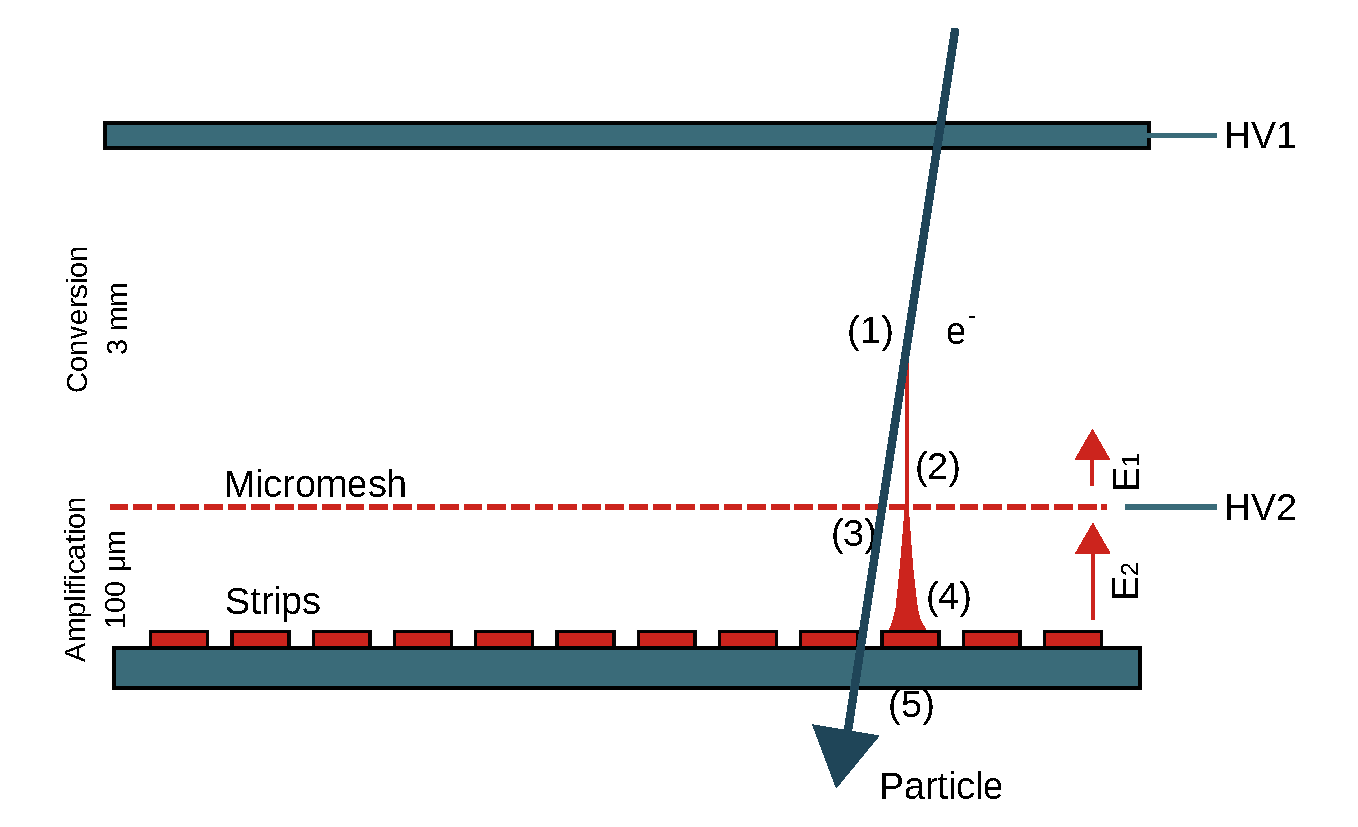
\includegraphics[width=\textwidth]{10mm_principle.pdf}}
        \caption[MM working principle.]{Micromegas working principle.
        Source: Re-render of original illustration by \cite{giomataris1996} using \href{https://inkscape.org/}{Inkscape}.}
        \label{fig::12.10::micromegas_principle}
    \end{figure}

    A Micro-Mesh Gaseous Detector or Micromegas (MM) is a gaseous particle detector that is derived from wire chambers.
    These types of detectors are commonly used in experimental physics for detecting ionising particles.
    The MM detector offers very precise temporal and spatial resolution, on the order of 100 nanoseconds and below 100 micrometers \cite{giomataris1996}.

    The detector operates by amplifying the charges created by ionisation in the gas volume.
    Its volume is divided into two parts by a metallic micro-mesh placed less than 150 micrometers away from the readout electrode or strip.

    To illustrate this process, refer to Figure \ref{fig::12.10::micromegas_principle}.

    When a particle passes through the detector, it ionises the gas atoms by stripping an electron, resulting in an electron-ion pair (1).
    An electric field, denoted as $\text{E}_1$, is applied to the gas, causing the electron to drift towards the amplification electrode (2) while the ion moves towards the cathode.
    As the electron crosses the mesh (3), it enters a strong electric field, denoted as $\text{E}_2$, triggering an avalanche effect (4).
    This produces a significant signal at the readout strip (5), which can then be stored for reconstruction \cite{giomataris1996}.

% --+ Micromegas in CLAS12 +----------------------------------------------------
    Inside the CLAS12 detector, a diverse set of tracking detectors is utilised to determine the positions and momenta of particles at different points along their trajectories.
    The proximity of these detectors to the particle source directly correlates to the precision achieved in determining the position and momentum at the interaction vertex, which refers to the point where the particle was generated.
    To optimise this precision, the Micromegas Vertex Tracker (MVT) is positioned as close as feasible to the target, as depicted in Figure \ref{fig::12.10::micromegas_vertex_tracker}.

    \begin{figure}[b!]
        \centering\frame{
        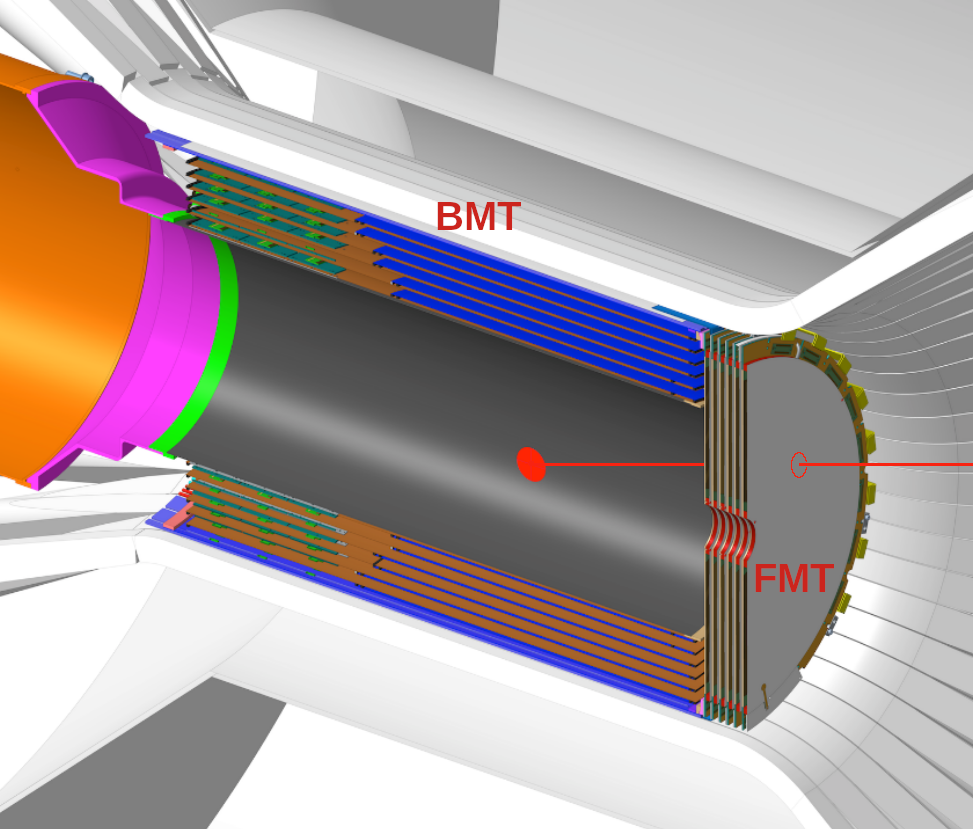
\includegraphics[scale=0.5]{10mvt.png}}
        \caption[MVT detector.]{MVT detector.
        The red dot denotes the $z=0$ point in the beamline, the red line denotes an arbitrary track coming from that point, and the circumference in the FMT denotes where that track produces a signal in an FMT layer.
        Source: \href{https://jlab.org/physics/hall-b/clas12}{CLAS12 wiki}.}
        \label{fig::12.10::micromegas_vertex_tracker}
    \end{figure}

    Similar to the division of CLAS12 into the CD and FD, the MVT is also divided into two parts to maximise the angular coverage.

    The first component is the BMT, which consists of 18 cylindrical detectors arranged in 6 layers.
    When combined with the SVT, this detector covers the angular region from $35$ to $125$ degrees, significantly enhancing the resolution of the polar angle \cite{acker2020mvt}.

% --+ FMT +---------------------------------------------------------------------
    Then, the FMT, which is made of six circular, flat detectors covering angles from $6$ to $29\degree$.
    In theory, it should improve the vertex resolution by a factor of $3$ to $10$ when compared to the DC \cite{aune2009}.
    While the original design of the FMT included six layers, the current implemented detector has only three layers installed.
    This is due to technical difficulties and concerns regarding its Lorentz angle \cite{konczykowski2010}.

    Each of the three FMT layers has $1024$ readout strips, which follow a peculiar distribution, as can be seen in the image to the right of Figure \ref{fig::12.10::fmt_geometry}.
    In addition, each layer's orientation differs by $60\degree$ to provide an accurate measurement in the xy-plane, as is shown in the image at the centre of the same Figure \cite{acker2020mvt}.

    \begin{wrapfigure}{r}{0.50\textwidth}
        \centering\frame{
        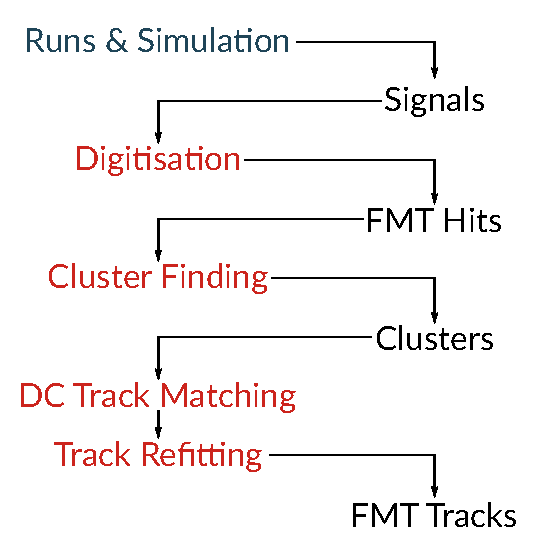
\includegraphics[width=\linewidth]{10fmt_recon.pdf}}
        \caption[FMT reconstruction summary]{FMT reconstruction summary.
        Data taking is coloured blue, data in black, and processes in red.
        Source: Own elaboration, using \href{https://inkscape.org/}{Inkscape}.}
        \label{fig::12.11::fmt_reconstruction}
    \end{wrapfigure}

    The FMT is composed of six circular, flat detectors that cover angles ranging from $6$ to $29$ degrees.
    In its conception, it was anticipated that the FMT would improve the vertex resolution by a factor of 3 to 10 compared to the DC \cite{aune2009}.
    However, the currently implemented FMT deviates from the original design, with only three layers installed.
    This modification was necessitated by technical difficulties and concerns related to its Lorentz angle \cite{konczykowski2010}.

    Each of the three FMT layers is equipped with 1024 readout strips that exhibit a distinctive distribution, as depicted in the image on the right-hand side of Figure \ref{fig::12.10::fmt_geometry}.
    Additionally, the orientation of each layer differs by 60 degrees to ensure accurate measurements in the xy-plane, as illustrated in the image at the center of the same Figure \cite{acker2020mvt}.

    \begin{figure}[t]
        \centering\frame{
        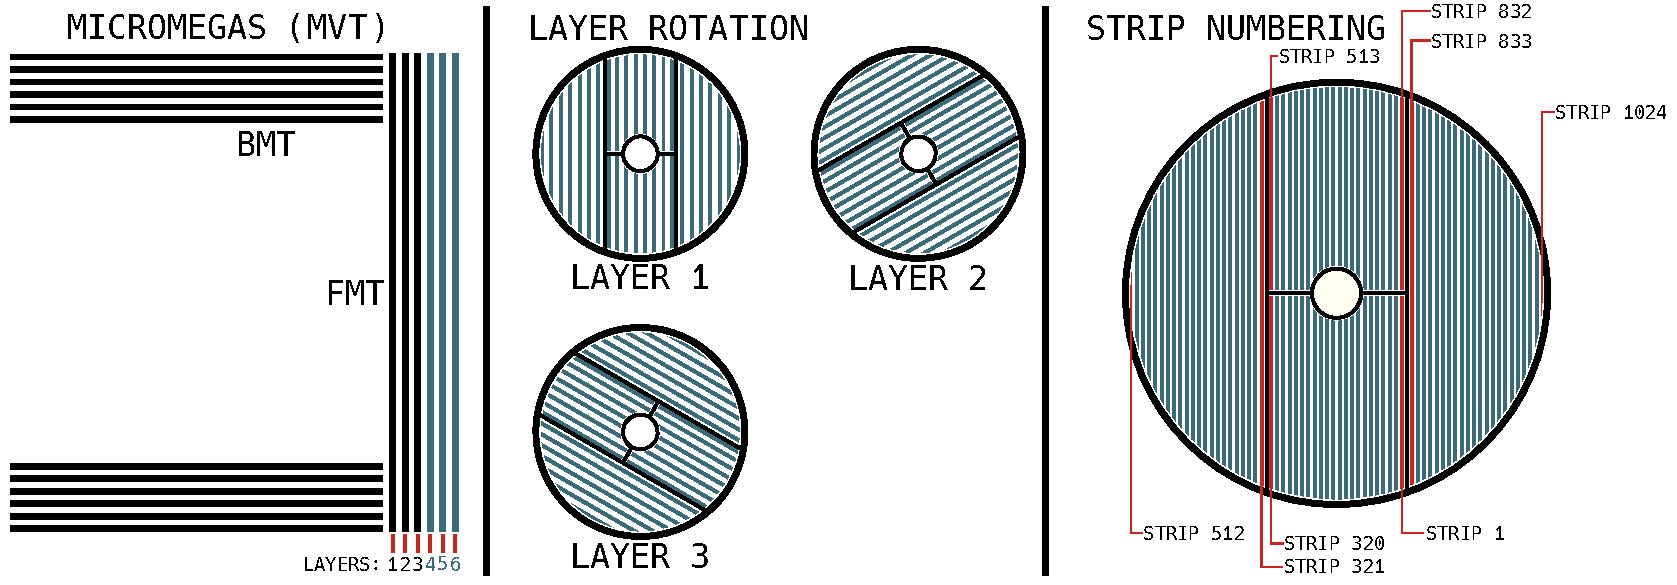
\includegraphics[width=\textwidth]{10fmt_geometry.pdf}}
        \caption[FMT detector geometry.]{FMT detector geometry. The first picture shows the distribution of the BMT and FMT layers, the second the different angle of each FMT layer, and the third the readout strip distribution of each FMT layer.
        Source: Own elaboration, using \href{https://inkscape.org/}{Inkscape}.}
        \label{fig::12.10::fmt_geometry}
    \end{figure}

    % !TEX root = ../main.tex
\subsubsection{FMT Track Reconstruction}
\label{sssec::fmt_track_reconstruction}
    Once a signal is detected on a readout strip and the data is stored, the information is extracted from it during offline reconstruction.
    The reconstruction process of the FMT closely resembles that of the DC.

    To begin with, when a signal is detected in a strip, it undergoes digitisation, processing, and is transformed into an \textbf{FMT Hit}.
    A set of FMT hits is then processed using a \textbf{Cluster Finding} algorithm, where a \textbf{Cluster} is defined as a group of hits that likely originate from the same particle track.
    Groups of clusters from different layers are subjected to a \textbf{DC Track Matching} algorithm, where they are matched to DC tracks generated by the DC Reconstruction process.
    Subsequently, a \textbf{Track Refitting} algorithm is employed for each DC track using the data from the clusters, resulting in updated tracks known as \textbf{FMT tracks}.
    An overview of this entire process is provided in Figure \ref{fig::fmt_recon}.

